\documentclass[ruledheader,noindentfirst,anapcustomindent,abntfigtabnum,tocpage=plain]{abnt}
\usepackage{amsmath, amssymb, amsthm, verbatim, amsfonts, amstext}
%\usepackage[latin1]{inputenc}
\usepackage[brazilian]{babel}
\usepackage[utf8]{inputenc}
\usepackage[T1]{fontenc}
\usepackage{dropping}
\usepackage{graphicx}
\usepackage[hang,small,bf]{caption}
\usepackage[abnt-etal-list=0,abnt-etal-text=it,abnt-and-type=&,abnt-emphasize=bf,abnt-full-initials=yes,alf,bibjustif]{abntcite}
\usepackage{fancyhdr}
\usepackage{makeidx}
\usepackage[none]{hyphenat}
\usepackage{color}
\usepackage{subfig}
\usepackage{algorithms}
\usepackage{algorithmic}
\usepackage{mdwlist}
\usepackage{bm}
\usepackage[titletoc,title]{appendix}
\usepackage{ltxtable}
\usepackage{longtable}
\usepackage{supertabular}
\usepackage{indentfirst}
\usepackage{color}
\usepackage{icomma}

\sloppy


%
%Tradução do pacote Algorithm para portugues
%
\renewcommand{\algorithmicrequire}{\textbf{Entrada:}}
\renewcommand{\algorithmicensure}{\textbf{Saída:}}
\renewcommand{\algorithmicend}{\textbf{fim}}
\renewcommand{\algorithmicif}{\textbf{se}}
\renewcommand{\algorithmicthen}{\textbf{então}}
\renewcommand{\algorithmicelse}{\textbf{senão}}
\renewcommand{\algorithmicelsif}{\algorithmicelse \, \algorithmicif}
\renewcommand{\algorithmicendif}{\algorithmicend \, \algorithmicif}
\renewcommand{\algorithmicfor}{\textbf{para}}
\renewcommand{\algorithmicforall}{\textbf{para todo}}
\renewcommand{\algorithmicdo}{\textbf{fazer}}
\renewcommand{\algorithmicendfor}{\algorithmicend \, \algorithmicfor}
\renewcommand{\algorithmicwhile}{\textbf{enquanto}}
\renewcommand{\algorithmicendwhile}{\algorithmicend \, \algorithmicwhile}
\renewcommand{\algorithmicloop}{\textbf{laço}}
\renewcommand{\algorithmicendloop}{\algorithmicend \, \algorithmicloop}
\renewcommand{\algorithmicrepeat}{\textbf{repetir}}
\renewcommand{\algorithmicuntil}{\textbf{até}}
\renewcommand{\algorithmiccomment}[1]{\{#1\}}
\renewcommand{\listalgorithmname}{Lista de Algoritmos}
\floatname{algorithm}{Algoritmo}
%%%%%%%%%%%%%%%%%%%%%%%%%%%%%%%%%%%%%%%%%%%%%%%%%%%%%%%%%%%%%%%%%%%%%%%%%%%%%%%%%%%

\makeindex

%%%% O arquivo modelosCAP.tex possui as definições para ciação do estilo de capítulo (fonte de título, barras horizontais, etc.)
% ele não gera texto de saída, é um arquivo de configuração somente
%
%Estilo de formatação de capítulos

\makeatletter
\newcommand{\thechapterwords}
{ \ifcase \thechapter\or 1\or 2\or 3\or 4\or 5\or6\or 7\or 8\or 9\or 10\or 11\fi}

\def\@makechapterhead#1{%
\vspace*{10\p@}%
{\parindent \z@  \reset@font

\scshape \@chapapp{} \thechapterwords
\quad %
\par\nobreak
\vspace*{10\p@}%
\interlinepenalty\@M
\hrule
\vspace*{10\p@}%
\Huge \bfseries #1\par\nobreak
\par
\vspace*{10\p@}%
\hrule
\vskip 40\p@
}}
\def\@makeschapterhead#1{%
\vspace*{10\p@}%
{\parindent \z@ \centering \reset@font
\par\nobreak
\vspace*{10\p@}%
\interlinepenalty\@M
\hrule
\vspace*{10\p@}%
\Huge \bfseries #1\par\nobreak
\par
\vspace*{10\p@}%
\hrule
\vskip 40\p@
%\vskip 100\p@
}}
%%%%%%%%%%%%%%%%%%%%%%%%%%%%%%%%%%%%%%%%%%%%%%%FIM DO PREAMBULO%%%%%%%%%%%%%%%%%%%%%%%%%%%%%%%%%%%%%%%%%%%%%%%%%%%%%%%%%%%%%%%%%%


\begin{document}

%%%%% IMPORTANTE: ALTERA O TEXTO ENTRE ARIAL E TIMES NEW ROMAN (ALTERNAR OS COMENTÁRIOS)
%
%%%%%%%%%%%%%%%%%%%%%PARA UTILIZAR ARIAL%%%%%%%%%%%%%%%%%%%%%%%
%
\fontfamily{phv}                    %fonte Arial
\renewcommand{\rmdefault}{phv}      %
%
%%%%%%%%%%%%%%%%%%%%%PARA UTILIZAR TIMES%%%%%%%%%%%%%%%%%%%%%%%
%
%\fontfamily{ptm}               %fonte Times
%\renewcommand{\rmdefault}{ptm} %
%
%%%%%%%%%%%%%%%%%%%%%%%%%%%%%%%%%%%%%%%%%%%%%%%%%%%%%%%%%%%%%%%

%%%%%%%%%%%%%Arquivos .tex com os elementos pré-textuais
%
\thispagestyle{empty}

\vfill
 \begin{center}
    \begin{figure}[t]
     \centering
            
\includegraphics[width=5cm]{figures/IF_logo.eps}\\[-0.1in]
     \end{figure}

    {\large\bfseries INSTITUTO FEDERAL DE EDUCAÇÃO, CIÊNCIA E TECNOLOGIA DO CEARA} \\
    {\large\bfseries PRÓ-REITORIA DE ENSINO} \\
    {\large\bfseries COORDENADORIA DE TELEMÁTICA DO CAMPUS MARACANAÚ}  \\ 
    {\large\bfseries BACHARELADO EM CIÊNCIA DA COMPUTAÇÃO}  \\ 

    \vspace*{1in}
    \begin{large} \bfseries FELIPE MARCEL DE QUEIROZ SANTOS \end{large}\\[0.4in]

    \vspace*{4cm}
    \noindent \\
    \large\bfseries{TÍTULO DO TRABALHO} \\
    \vfill
    \large\bfseries{ MARACANAÚ \\ 2015}
\end{center}

\normalsize
\begin{titlepage}
\vfill
\begin{center}

    {\large MAYANNA RODRIGUES FERREIRA\\}
    \vspace{2cm}
    {\Large \textsc{CONSTRUINDO UM PERFIL DO CONSUMO ENERGÉTICO DE ALGORITMOS EM UMA PLATAFORMA EMBARCADA}\\}
    \vspace{1cm}
    \hspace{.45\linewidth}
    \begin{minipage}{.50\linewidth}

            Monografia submetida à Coordenadoria de Telemática e à Coordenadoria do Curso de Bacharelado 
            em Ciência da Computação do Instituto Federal do Ceará - Campus Maracanaú, como requisito 
            parcial para obtenção do grau de Bacharel em Ciência da Computação.

            \vspace{0.5 cm}

            Área de pesquisa: Sistemas Embarcados 
            

            \vspace{0.5 cm}

            Orientador: Dr. Otávio Alcântara de Lima Junior 
    
    \end{minipage}

    \vspace{2cm}
    \vfill
    {\large Maracanaú\\ 2020}
\end{center}

\end{titlepage}
\begin{folhadeaprovacao}
\setlength{\ABNTsignthickness}{0.2pt}
\setlength{\ABNTsignskip}{1.7cm}

\begin{center}

\includegraphics[width=2.5cm]{figures/brasao_republica.eps}\\
%
\includegraphics[width=5cm]{figures/IF_logo.eps}\\ %outros brasões
%
\includegraphics[width=5cm]{figures/IF_logo2.eps}\\%outros brasões

            {INSTITUTO FEDERAL DE EDUCAÇÃO, CIÊNCIA E TECNOLOGIA DO CEARÁ} \\
            {COORDENAÇÃO DE PÓS-GRADUAÇÃO EM ENGENHARIA DE TELECOMUNICAÇÕES}  \\

    \vspace{1.5cm}
                                    {FELIPE MARCEL DE QUEIROZ SANTOS}\\
    \bfseries{}
\end{center}

Esta Monografia foi julgada adequada para a obten\c{c}\~{a}o do Grau de Bacharel em Ciência da Computação, sendo aprovada pela Coordenadoria de Telemática e pela Coordenadoria do curso de Bacharelado em Ciência da Computação do Campus Maracanaú do Instituto Federal de Educação, Ciência e Tecnologia do Ceará e pela banca examinadora:

    \vspace{0.15cm}
    \assinatura{Orientador: Prof. Dr. Amauri \\ Instituto Federal do Ceará - IFCE}
    \assinatura{Prof. Dr. Huguinho \\ Instituto Federal do Ceará - IFCE}
    \assinatura{Prof. Dr. Zezinho \\ Instituto Federal do Ceará - IFCE}
    \assinatura{Prof. Dr. Luizinho \\ Instituto Federal do Ceará - IFCE}
    \vspace{0.15cm}%\vfill

    \begin{center}
        Fortaleza, 06 de Abril de 2013
    \end{center}
\end{folhadeaprovacao}
\vspace*{15cm}

\hfill  {\itshape Para meus pais}\\
\chapter*{Agradecimentos}
%\thispagestyle{empty}


\begin{flushright}
\begin{minipage}[r]{10cm}
\vspace{18cm}
``A mente que se abre a uma nova idéia jamais voltará ao seu tamanho original''.
\begin{flushright}
Albert Einstein
\end{flushright}
\end{minipage}
\end{flushright}
\pagestyle{plain}%%%%% Utilizar ESTILO PLAIN AQUI%%%%%%%
\chapter*{Resumo}

\noindent A tecnologia está onipresente atualmente, isso se deve em muito por causa da internet
das coisa, já que  ela possibilitou a automatização de diversos equipamentos. Apesar dessa automação os equipamentos não ficaram totalmente independentes uma vez que ainda existe a dependência da eletricidade. Alguns desses equipamentos tem como fonte de energia bateria, que tem sua vida útil limitada, sendo assim conhecer o quanto será consumido de energia se torna imprescindível. Uma boa parte do consumo energético vem dos algoritmos que estão funcionando na plataforma. Atualmente já existem diversos modelos para se calcular o consumo energético de algoritmos em plataformas embarcadas, porém não são completamente eficientes, sendo assim a proposta seria juntar mais de um desses modelos para uma maior eficiência e precisão nas medições. Para realizar a experimentações o presente trabalho propõe explora uma plataforma chamada Repito
para que assim possa traçar o perfil do consumo de energia de alguns algoritmos
implementados em sistemas embarcados.



\textbf{Palavras-chaves}: Sistemas embarcados, perfil energético, internet das coisas.

\chapter*{Abstract}


\noindent The technology is ubiquitous today, this is due in large part because of the internet of things, since it enabled the automation of various equipment. many of those automation systems as a central platform for an embedded system. This work proposes to explore a platform called Repito so that it can outline the energy consumption profile of some algorithms implemented in embedded systems.
 
 \textbf{Keyword}: Embedded systems, energy profile, internet of things.

 

%%%Comandos para criação automática das listas
%
\tableofcontents
\listoffigures
\listoftables

%%%Comandos para criar outras listas não suportadas pelo pacote ABNTex%%%
%
\pretextualchapter{Lista de Símbolos}
\begin{basedescript}{\desclabelstyle{\pushlabel}\desclabelwidth{6em}}
\item[$Z$] variavel aleatoria%
\item[$\mathbb{R}$] conjunto dos números reais%
\item[$t$] tempo contínuo%
\item[$n$] tempo discreto%
\item[$f(z)$] função densidade de probabilidade%
\item[$F(z)$] função de distribuição acumulada%
\item[$\sigma$] desvio padrão%
\item[$\mu$] média ou esperança matemática%
\item[$|\cdot|$] operador magnitude%
\item[$\nabla$] operador gradiente%
\end{basedescript}
\newpage

\pretextualchapter{Lista de Abreviacoes}
\begin{basedescript}{\desclabelstyle{\pushlabel}\desclabelwidth{6em}}
\item[{fdp}] Função densidade de probabilidade%
\item[{fda}] Função de distribuição acumulada%
\item[{EMQ}] Erro médio quadrático%
\end{basedescript}
\newpage
%%%%%%%%%%%%%%%%%%%%%%%%%%%%%%%%%%%%%%%%%%%%%%%%%%%%%%%%%%%%%%%%%%%%

%Capítulos passam a ter páginas numeradas
%
\pagestyle{fancy}

%resseta os contadores de capítulo e seção
%
\renewcommand{\chaptermark}[1]{\markboth{#1}{}}
\renewcommand{\sectionmark}[1]{\markright{\thesection\ #1}}

%%%%%%%%%%%%%%NÃO LEMBRO O QUE FAZ, APARENTEMENTE NADA, TESTAR DEPOIS
%\fancyhf{}%
%\fancyhead[RO,LE]{\large\slshape\thepage}%
%\fancyhead[CE]{\large\slshape\leftmark}%
%\fancyhead[CO]{\large\slshape\rightmark}%


%%% Outros arquivos .tex. É acoselhável utilizar vários arquivos, pelo menos um por capítulo
\chapter{Introdução}\label{CAP:introducao}
%\thispagestyle{empty}

A tecnologia está cada vez mais presente na vida da sociedade atual. As evoluções dessas tecnologias nas últimas décadas foram enormes. Hoje, elas estão presentes em diversos âmbitos da sociedade, como na agricultura, no comércio, nos equipamentos médicos, no monitoramento de rodovias, nas casas e até no corpo humano. Nesse cenário, os sistemas embarcados tornam-se cada vez mais presentes no cotidiano.

Os sistemas embarcados têm muitas características que os beneficiam, tais quais: o preço acessível, a portabilidade e a capacidade de processamento, que só vem aumentando com o passar dos anos, além do baixo consumo de energia. 
            
Muitos desses equipamentos irão passar longos períodos sem nem uma intervenção humana. Sendo assim, apesar de seu pequeno consumo de energia, é muito importante ter uma noção exata de quanto ele será, para que, dessa forma, seja possível aumentar a autonomia do sistema e, consequentemente, sua vida útil. O consumo de energia desses dispositivos pode variar muito em função das operações atreladas a aplicação, dos modos de operação e dos periféricos utilizados. O que também pode contribuir para o gasto energético são os softwares utilizados no sistema.	
      
\section{Motivaçâo}
Diante da proeminente proliferação dos sistemas embarcados na sociedade e de todos os desafios existentes para torná-los mais eficientes quanto ao consumo energético, torna-se necessário ter conhecimento do perfil energético de determinados algoritmos que nos dispositivos serão utilizados. Com a construção dos perfis energéticos, seria mais fácil comparar e decidir qual algoritmo utilizar em determinados dispositivos e situações e, por consequência, o sistema desenvolvido seria mais eficiente.

\section{Objetivo Geral}
Traçar, de forma consistente, um perfil de consumo de energia de alguns algoritmos em um sistema embarcado em diferentes situações, permitindo, assim, uma avaliação apurada para uso em plataformas de simulação.

\subsection{Objetivos Especificos}
Os objetivos específicos deste trabalho são os seguintes:
\begin{itemize}
    \item 	Utilizar a plataforma apresentada no artigo {\itshape An FPGA-based evaluation platform for energy harvesting embedded systems} (ALCÂNTARA; DE LIMA; FURTADO, 2019) para fazer os experimentos;
    
    \item 	Empregar os perfis de consumo de energia gerados em diferentes condições, para uso como fonte de dados para simulações;
     
     \item 	Comparar os perfis de consumo de um mesmo algoritmo em diferentes condições.

\end{itemize}



\section{Organizacao da tese}

Esta dissertação encontra-se estruturada da seguinte forma: este primeiro capítulo
trata da contextualização do tema, aponta o objetivo geral e os específicos do trabalho;
no segundo capítulo, será apresentada a fundamentação teórica necessária ao desenvolvimento do projeto, sendo descritos os conceitos relacionados a consumo energetico; a descrição da solução proposta será detalhada no terceiro capítulo;
\chapter{Fundamentação teórica}
\label{CAP2}


Neste capítulo são apresentadas algumas formas de construir um perfil de consumo energético de algoritmos implementados em sistemas embarcados com exemplos de casos de usos e algumas técnicas de calcular o consumo de energia de algoritmos. Por fim, é apresentada uma técnica de emulação de captura de energia detalhando suas especificidades.


\section{Sistemas embarcados}
 A enorme de evolução dos sistemas embarcados fez com que a sociedade se tornar, de certa forma, dependente deles. Um Sistema Embarcado pela sua natureza especialista, pode ter inúmeras aplicações (CHASE, 2007). Aplicações, essa que vão desde o setor automotivo até a medicina chegando até mesmo ao vestuário. O avanço da tecnologias, em especial as digitais, irá afetar profundamente todas as estruturas econômicas e sociais, talvez a mais impactante e pervasiva dessas tecnologias digitais seja
a internet das coisas, objeto de atenção prioritária de governos e da iniciativa privada pelo mundo inteiro (MAGRANI, 2018).  O IoT ainda deve crescer muito nos próximos anos como mostra graficamente a Figura 1 da IHS (2016).  
\begin{figure}[!ht]
\centering
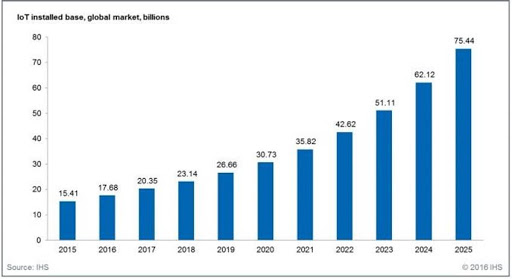
\includegraphics[scale=.65]{figures/grafico.jpg}
\caption{ Figura 1 - The IoT market will be massive. Fonte IHS (2016) } \label{Fig:1}
\end{figure}

Os avanços da microeletrônica proporcionaram o surgimento de diversos microprocessadores, microcontroladores, processadores de sinais digitais (DSP) e FPGA baseado em VLSI. Esse dispositivos estão presentes principalmente em dentro de outros dispositivos, sendo assim eles não são isíveis para o usuário ou seja são Ubíquos. Por seu baixo custo, desempenho satisfatório e em geral tamanho pequeno eles são sempre cotados para diversas aplicações. Não é atoa que os sistemas embarcados sejam os queridinhos do IoT, construir redes de comunicações inteiras entre dispositivos só se fez possível por causa deles. Eles também são responsaveis pelo processamento digital de divesos sinais.           



Cada um desses  microeletrônicos tem suas peculiaridades porém todos eles têm algo, muito nítido, em comum eles depende de energia para seu funcionando.Como estes sistemas são largamente usados em dispositivos que utilizam baterias como fonte de energia eles  devem ter consumo energético bastante restrito (NETO, et al. 2010). 
 Saber quanto é seu consumo energético se torna importante para seu total aproveitamento, uma parte desse consumo vem do algoritmo que está implementado no sistema. Para saber o consumo energético de determinados algoritmos existem alguns métodos que serão abordados a seguir.

\section{Métodos para calcular o consumo energético}

\subsection{Modelos Matematicos}
Construir um modelo matemático que possa determinar o desempenho energético um sistema sem que ele esteja montado fisicamente seria muito interessante, já que assim simplificaria e muito o processo de produção. Um modelo com essas características já foi construído para redes de sensores sem fio. O modelo proposto aborda uma parte importante do processo operacional das redes de sensores visuais sem fio, que é o processamento interno nos nós sensores (CERQUEIRA; COSTA, 2019).

\subsection{Simuladores}
Existem alguns simuladores de consumo energético um desse é o Sim-Panalyzer.  O SimpleScalar é um simulador de arquitetura computacional que modela um computador virtual com CPU, cache e hierarquia de memória e com base nesse modelo consegue simular programas reais executando sobre a plataforma especificada (LIMA; et al., 2012).

\subsection{Osciloscópio }
Dentre de todos os métodos relatados acima o osciloscópio é o mais tradicional quando se trata de medição de consumo de energia. Para a medição do consumo de energia foi usado o osciloscópio para medir a corrente consumida pelo processador ao executar o algoritmo desejado. Para medir a corrente, foi inserido um resistor de 0.333 Ohm conectado em série com o cabo de alimentação ATX12V da placa mãe e medida a diferença de voltagem da entrada e saída do resistor de shunt que foi inserido em série no circuito da placa principal,conforme se observa na Figura 2 ( NETO; MORENO; MATOS, 2011) .

\begin{figure}[!ht]
\centering
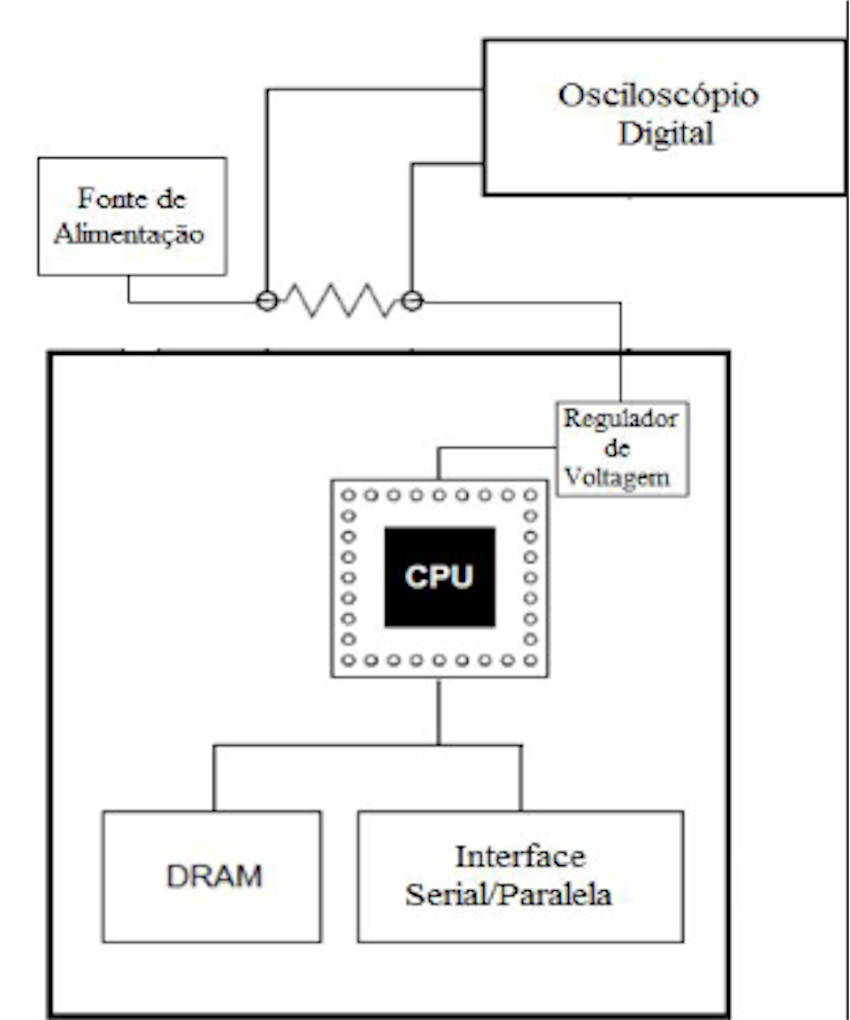
\includegraphics[scale=.65]{figures/ociloscopio.png}
\caption{ Figura 2 - Esquema utilizado para as medições com o Osciloscópio. Retirado de  ( Neto; Moreno; Matos, 2011). } \label{Fig:1}
\end{figure}


\section{Ripeto}
 Ripeto, uma plataforma de avaliação para EHES que pode imitar o comportamento do transdutor de captação de energia e registrar em rastreamentos de energia de memória e dados do analisador lógico para assegurar adequadamente o desempenho de um EHES (ALCANTARA; DE LIMA; FURTADO, 2019). O Ripeto é baseado em um FPGA Sparten6, da Xilinx, com 32 Mb de memória de DRAM acoplada.

\begin{figure}[!ht]
\centering
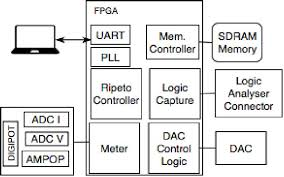
\includegraphics[scale=.65]{figures/ripeto.png}
\caption{Figura 3 - Arquitetura da Plataforma. Retirado de (ALCANTARA; DE LIMA; FURTADO, 2019) } \label{Fig:1}
\end{figure}

O elemento central, o FPGA é onde os  componentes lógicos são implementados. A intenção com essa plataforma é capturar os  perfis de fornecimento de energia de fontes renováveis e reproduzi los de forma consistente. O Ripeto é um excelente sistema embarcado para a realização dos experimentos deste trabalho, já que ele é uma plataforma embarcada com uma certa limitação energética. Sendo assim, ele foi escolhido para a realização dos experimentos do projeto.  
 


\chapter{Método Proposto}\label{CAP3}
 Neste capítulo, são detalhados como os conceitos teóricos da seção anterior são colocados em prática na elaboração do que proposto. O estudo baseia-se fundamentalmente nos manuais dos fabricantes dos modelos dos microcontroladores escolhidos e no artigo {\itshape An FPGA-based evaluation platform for energy harvesting embedded systems} (ALC NTARA; DE LIMA; FURTADO, 2019) para fazer os experimentos.  

Para comparação entre os diferentes métodos apresentados anteriormente será necessario os resultados dos experimentos, que  serão realizados com algoritmos e sistemas embarcados. Os algoritmos a serem utilizados poderam ser o Fast Fourier transform, uma convolução ou filtros FIR. 


\chapter{Cronograma}\label{CAP4}
Neste capítulo será apresentado o cronogranogra para realização o que foi proposto no capítulo anterior. A pesquisa deverá acontecer em um período de seis meses.   

\begin{table}[!hp]
\centering
   \caption{Cronograma de pesquisa}
   \label{tab:1}

\begin{tabular}{|c|c|}
 
	\hline
	Mês &  O que será feito\\
	\hline
   1 &  Levantamento bibliografico e elaboração do projeto\\
	\hline
   2 &  Implementação de algoritmo\\
	\hline
	  3 &  Realização de experimentos\\
	\hline  
	4 & Realização de experimentos\\
	\hline  
	5 &  Coleta de dados e elaboração dos perfis de consum\\
	\hline
	  6 & Redação do trabalho, revisão e entraga da monografia\\
	\hline
	
\end{tabular}
\end{table}
\chapter{Conclusão e Trabalhos Futuros}\label{CAP5}


%%%% Estilo de citação ABNT e arquivo de bibitens (mybibliography.bib)
\bibliographystyle{abnt-alf}
\bibliography{mybibliography}

\apendice
\chapter{Título do Apêndice}
\label{Apx:A}




\chapter{Exemplo do pacote Algorithm}
\label{Apx:B}


\begin{algorithm}[!h]
\caption{Estimador ML otimizado.}\label{Alg:MAXVER}
\begin{algorithmic}[1]
\STATE Inicializar o contador: $j\leftarrow 1$;%
\STATE Fixar o limiar de variação das estimativas: $e_{\mathrm{out}}\leftarrow 10^{-4}$;%
\STATE Fixar o número máximo de iterações: $N\leftarrow 1000$;%
\STATE Computar o ponto inicial: $\hat \gamma(0)$;%
\STATE Determinar o limiar inicial: $e_1 \leftarrow1000$;%
\STATE Estabelecer o valor inicial de $\alpha$: $\hat \alpha(0) \leftarrow -10^{-6}$;%
\WHILE{ $e_j \geq e_{\mathrm{out}}$ e $ j\leq M$}
    \STATE Solucionar $\hat \alpha_j\leftarrow {\arg \max}_{\alpha}\;{l_1(\alpha; \gamma_{j-1},\mathbf{z},n)}$;%
    \STATE Solucionar $\hat \gamma_j\leftarrow {\arg \max}_{\gamma}\;{l_2(\gamma; \alpha_j,\mathbf{z},n)}$;%
    \STATE $j\leftarrow j+1$
    \STATE Computar o critério de convergência: $e_j$;%
\ENDWHILE
\end{algorithmic}
\end{algorithm}


\end{document}